\documentclass[tikz,border=10pt]{standalone}
\usepackage{pgfplots}
\usetikzlibrary{decorations.pathmorphing, arrows.meta, positioning, calc}

\begin{document}
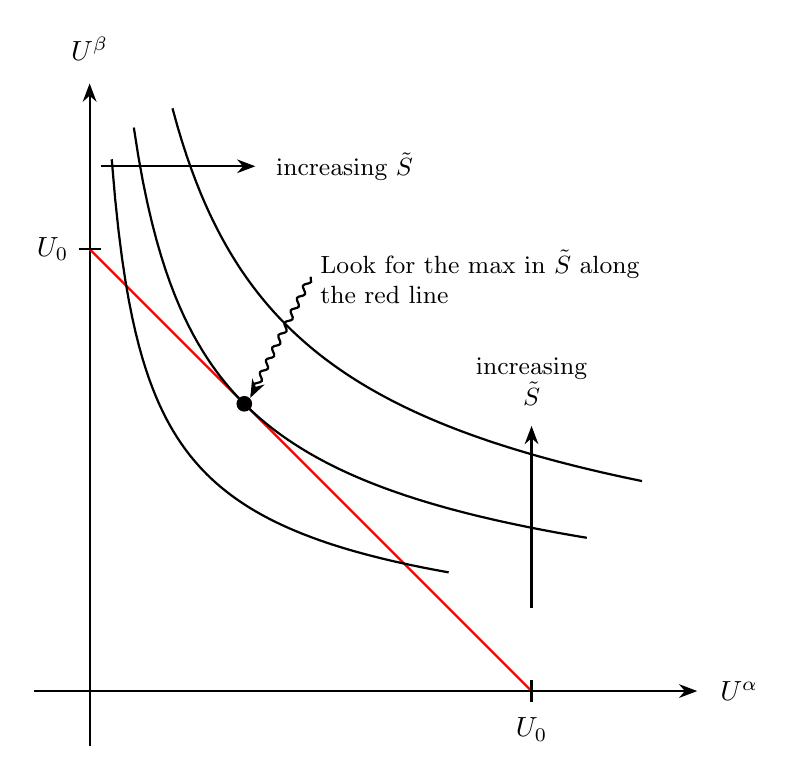
\begin{tikzpicture}
    \begin{axis}[
        % --- Axis Setup ---
        axis lines = middle,
        xlabel = {$U^\alpha$},
        ylabel = {$U^\beta$},
        xlabel style = {at={(ticklabel* cs:1.02)}, anchor=west},
        ylabel style = {at={(ticklabel* cs:1.02)}, anchor=south},
        axis line style = {-Stealth, thick},
        % Domain view
        xmin = -1, xmax = 11,
        ymin = -1, ymax = 11,
        ticks = none,
        clip = false,
        width = 10cm,
        height = 10cm
    ]

        % --- Constants ---
        \def\Uzero{8}
        % Tangency point
        \def\TangentX{2.8} 
        \def\TangentY{5.2}
        
        % Calculate exponent 'n' for y = A/x^n
        \def\Power{0.538}
        
        % Calculate Coefficient A = y * x^n for the tangent curve
        \def\CoeffM{\TangentY * \TangentX^\Power}
        
        % Coefficients for lower and higher curves
        \def\CoeffL{0.65 * \CoeffM} 
        \def\CoeffH{1.45 * \CoeffM}

        % --- 1. Red Constraint Line ---
        \draw[red, thick] (axis cs:0, \Uzero) -- (axis cs:\Uzero, 0);
        
        % Ticks and Labels for U0
        \draw[thick] (axis cs: -0.2, \Uzero) -- (axis cs: 0.2, \Uzero) node[left=8pt] {$U_0$};
        \draw[thick] (axis cs: \Uzero, -0.2) -- (axis cs: \Uzero, 0.2) node[below=10pt] {$U_0$};

        % --- 2. Entropy Contours (Black Curves) ---
        % Adjusted domains to keep the graph clean
        
        % Lower Curve
        \addplot[thick, black, domain=0.4:6.5, samples=100] {\CoeffL / x^\Power};
        
        % Middle Curve (Tangent)
        \addplot[thick, black, domain=0.8:9, samples=100] {\CoeffM / x^\Power};
        
        % Higher Curve
        \addplot[thick, black, domain=1.5:10, samples=100] {\CoeffH / x^\Power};

        % --- 3. Tangency Point ---
        \node[circle, fill=black, inner sep=2pt] (maxpt) at (axis cs:\TangentX, \TangentY) {};

        % --- 4. Annotations ---
        
        % Squiggly Arrow Label
        % Moved slightly right to avoid overlap with the middle curve
        \node[align=left, font=\small, anchor=west] (lbl_max) at (axis cs: 4.0, 7.5) {
            Look for the max in $\tilde{S}$ along\\
            the red line
        };
        \draw[->, >=Stealth, thick, decorate, decoration={snake, amplitude=1pt, segment length=5pt, post length=3pt}] 
            (lbl_max.west) -- (maxpt.north east);

        % Top Left "Increasing S" (Horizontal)
        % Positioned to the left of the curves
        \node[anchor=west, font=\small] at (axis cs: 3.2, 9.5) {increasing $\tilde{S}$};
        \draw[->, >=Stealth, thick] (axis cs: 0.2, 9.5) -- (axis cs: 3.0, 9.5);
        
        % Bottom Right "Increasing S" (Vertical)
        % Positioned in the empty space on the right
        \node[anchor=south, font=\small, align=center] at (axis cs: 8.0, 5.0) {increasing \\ $\tilde{S}$};
        \draw[->, >=Stealth, thick] (axis cs: 8.0, 1.5) -- (axis cs: 8.0, 4.8);
        
    \end{axis}
\end{tikzpicture}
\end{document}